
\documentclass{standalone}
\usepackage[svgnames]{xcolor}
\usepackage{pgfplots}
\pgfplotsset{compat=newest}
\usepackage[sfdefault]{FiraSans}
\usepackage{FiraMono}
\renewcommand*\familydefault{\sfdefault}
\begin{document}
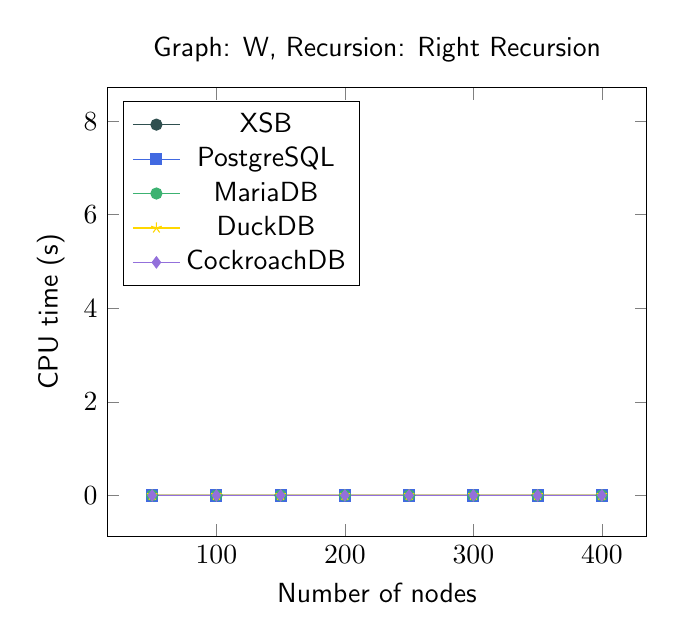
\begin{tikzpicture}
    \begin{axis}[
        title={Graph: W, Recursion: Right Recursion},
        xlabel={Number of nodes},
        ylabel={CPU time (s)},
        legend pos={north west},
        ymax=8.712522
    ]
    \addplot+[DarkSlateGray, mark options={color=DarkSlateGray}] coordinates {(50,0.00011050000000000105) (100,0.000316500000000001) (150,0.0004790000000000035) (200,0.0005970000000000005) (250,0.0007300000000000015) (300,0.0011340000000000026) (350,0.001179) (400,0.0015580000000000051)};
\addlegendentry{XSB}
\addplot+[RoyalBlue, mark options={color=RoyalBlue}] coordinates {(50,0.00011885000000000367) (100,0.00012199999999998323) (350,0.00013770000000001836) (300,0.0001481000000000121) (400,0.0001492999999999911) (200,0.0001554999999999751) (250,0.00016805000000000292) (150,0.00017955000000000054)};
\addlegendentry{PostgreSQL}
\addplot+[MediumSeaGreen, mark options={color=MediumSeaGreen}] coordinates {(400,0.00010835000000000705) (50,0.00011050000000001337) (150,0.00011559999999999349) (350,0.00011585000000002843) (250,0.00011659999999999449) (200,0.00012899999999999023) (300,0.00013670000000001736) (100,0.00014279999999997073)};
\addlegendentry{MariaDB}
\addplot+[Gold, mark options={color=Gold}] coordinates {(350,0.004850400000000005) (150,0.004997399999999985) (200,0.005071900000000018) (50,0.005407250000000002) (100,0.005474199999999985) (250,0.0054923000000000055) (300,0.005807599999999996) (400,0.006644499999999998)};
\addlegendentry{DuckDB}
\addplot+[MediumPurple, mark options={color=MediumPurple}] coordinates {(400,0.00016864999999999242) (50,0.00018340000000000023) (300,0.0001946999999999366) (200,0.00019985000000000142) (150,0.00020480000000000498) (250,0.0002241999999998967) (100,0.0002422999999999731) (350,0.0002518499999999979)};
\addlegendentry{CockroachDB}

    \end{axis}
\end{tikzpicture}
\end{document}
